%\begin{center}
%	\textbf{B. Evidence by Decades}
%\end{center}

%\textbf{I. Baseline Sample}

\begin{figure}[H]
	\centering
	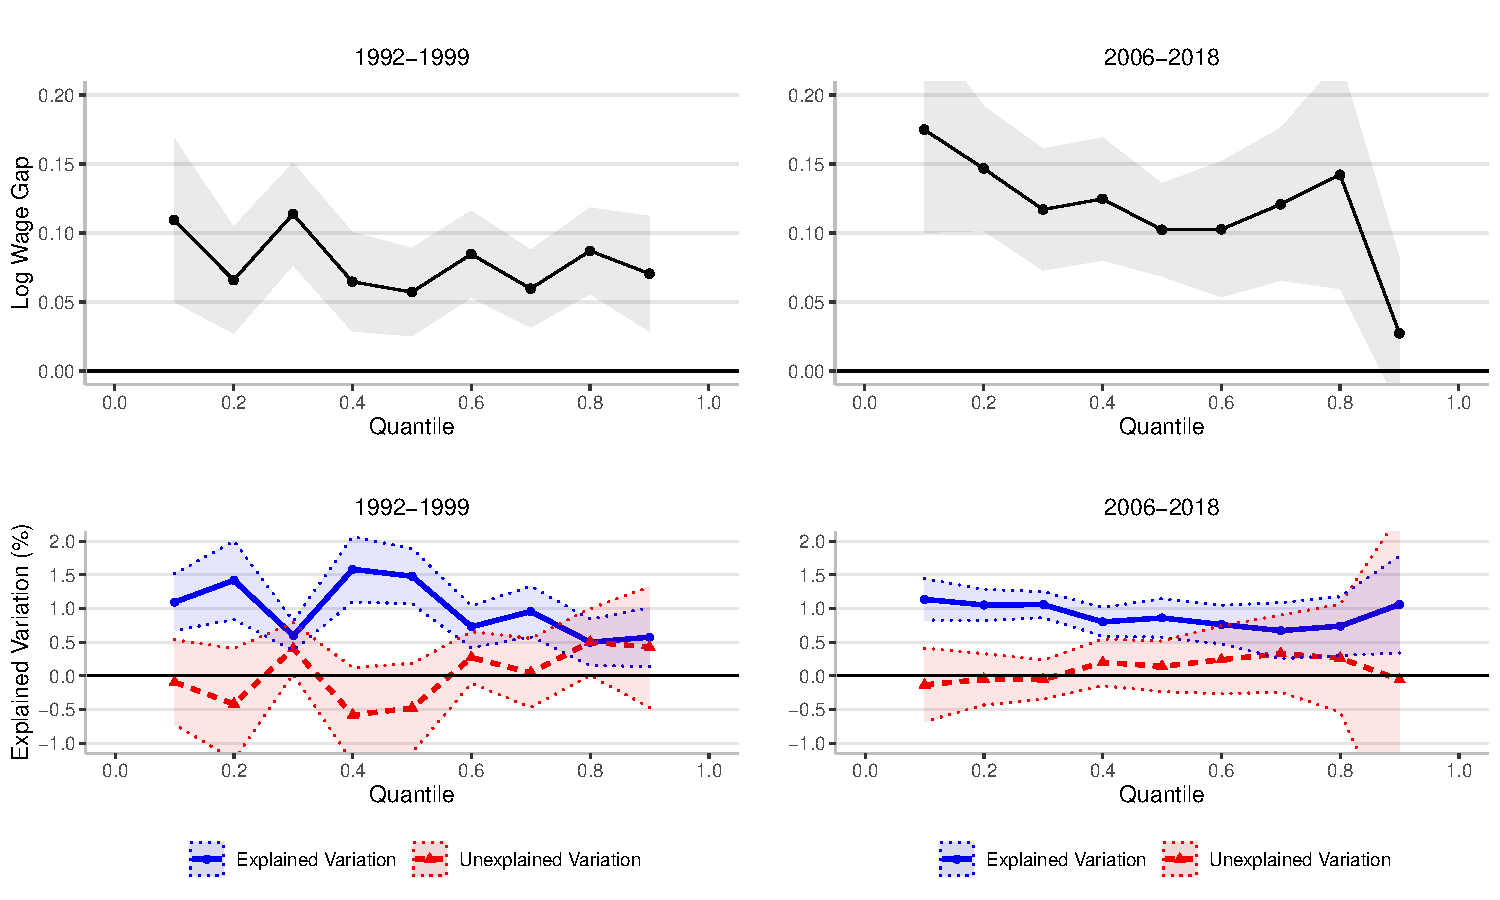
\includegraphics[width=1\linewidth]{nfgap_t}
	\caption{German Native-Foreign Wage Gap by sub-samples, 1992-2018 \label{fig:wgap_subs} \label{fig:wage_gap_base}}
	%	{\footnotesize NOTE. \textemdash The vertical difference between contributions from individual-level (``Indiv.'') variation in tasks and total variation (``Total'') reflects contributions from occupation-level variation in tasks. Therefore, the smaller this vertical gap, the more important is idiosyncratic variation relative to occupational variation .\par}
	%{\caption  {Contributions of Task Variation Within Occupations to the explained Native-Foreign Wage Gap with base task group Routine Manual, 1992-2018 \label{fig:wgap_within_baserm}}}
	
\end{figure}



\iffalse

\begin{figure}[H]
\centering
\begin{floatrow}
\ffigbox[\FBwidth]
{
\subfloat[Wage Gap: Distribution, 1992-1999 \label{fig:wgap90}]{\includegraphics[scale=0.25]{RIF_4_wgap90}} 
%RIF_5_wgap90
\quad
\subfloat[Wage Gap: Distribution, 2006-2018 \label{fig:wgap00}]{\includegraphics[scale=0.25]{RIF_4_wgap00}}
%RIF_5_wgap00 
}
{}
\end{floatrow}
\begin{floatrow}
\ffigbox[\FBwidth]
{
\subfloat[Explained Wage Gap, 1992-1999][Explained Wage Gap, 1992-1999 \label{fig:explained90}]{\includegraphics[scale=0.25]{RIF_4_ind_occ_task_immi3_90}} 
\quad
\subfloat[Explained Wage Gap, 2006-2018 \label{fig:explained00}][Explained Wage Gap, 2006-2018]{\includegraphics[scale=0.25]{RIF_4_ind_occ_task_immi3_00}} 
}
{}
\captionsetup{justification=centering}
{\caption{German Native-Foreign Wage Gap by sub-samples, 1992-2018 \label{fig:wgap_subs}}}
\end{floatrow}
%\bigskip
%{\footnotesize NOTE. \textemdash All point estimates are supplemented by a 95\% Confidence Interval (CI) based on bootstrapped standard errors with 100 replications.\par}
\end{figure}


\fi


